\documentclass[a4paper,12pt]{article}
\usepackage[left=1in, right=1in, top=1in, bottom=1in]{geometry}
\usepackage{placeins}
\usepackage{tikz}
\usetikzlibrary{trees}
\usepackage{graphics,graphicx}
\graphicspath{ {./images/} }
\usepackage{hyperref}
\usepackage[xindy,toc]{glossaries}

\usepackage{listings}
\usepackage{color}

\definecolor{dkgreen}{rgb}{0,0.6,0}
\definecolor{gray}{rgb}{0.5,0.5,0.5}
\definecolor{mauve}{rgb}{0.58,0,0.82}

% \lstset{frame=tb,
%   language=Java,
%   aboveskip=3mm,
%   belowskip=3mm,
%   showstringspaces=false,
%   columns=flexible,
%   basicstyle={\small\ttfamily},
%   numbers=none,
%   numberstyle=\tiny\color{gray},
%   keywordstyle=\color{blue},
%   commentstyle=\color{dkgreen},
%   stringstyle=\color{mauve},
%   breaklines=true,
%   breakatwhitespace=true,
%   tabsize=3
% }


% Taken from Lena Herrmann at 
% http://lenaherrmann.net/2010/05/20/javascript-syntax-highlighting-in-the-latex-listings-package

\definecolor{lightgray}{rgb}{.9,.9,.9}
\definecolor{darkgray}{rgb}{.4,.4,.4}
\definecolor{purple}{rgb}{0.65, 0.12, 0.82}

\lstdefinelanguage{JavaScript}{
  keywords={typeof, new, true, false, catch, function, return, null, catch, switch, var, if, in, while, do, else, case, break},
  keywordstyle=\color{blue}\bfseries,
  ndkeywords={class, export, boolean, throw, implements, import, this},
  ndkeywordstyle=\color{darkgray}\bfseries,
  identifierstyle=\color{black},
  sensitive=false,
  comment=[l]{//},
  morecomment=[s]{/*}{*/},
  commentstyle=\color{purple}\ttfamily,
  stringstyle=\color{red}\ttfamily,
  morestring=[b]',
  morestring=[b]"
}

\lstset{
   language=JavaScript,
   backgroundcolor=\color{lightgray},
   extendedchars=true,
   basicstyle=\footnotesize\ttfamily,
   showstringspaces=false,
   showspaces=false,
   numbers=left,
   numberstyle=\footnotesize,
   numbersep=9pt,
   tabsize=2,
   breaklines=true,
   showtabs=false,
   captionpos=b
}



\newcommand{\concatenate}{\mathbin{\|}}
\newcommand{\tablecell}[2][c]{%
  \begin{tabular}[#1]{@{}c@{}}#2\end{tabular}}
 
\makeglossaries

\newglossaryentry{Hash function}
{
  name={\ensuremath{H}, Hash function},
  description={In this paper, $H$ refers to the hash function. It takes in text
  and returns a Base64 string of the hash value of the string. The hash function used in XCredits is the SHA256Plus algorithm}
}

\newglossaryentry{SHA256Plus}
{
  name={SHA256Plus},
  description={SHA256Plus is a hash function that uses a SHA256 hash in two steps to prevent length extension attacks. See section \ref{SHA256Plus}
  }
}
  



\newglossaryentry{hash state}
{
  name={hash state},
  description={The hash state is the hash result of a block on a side shard. The hash state is communicated to the central chain to be included in the central chain blocks. 
  }
}

\newglossaryentry{microblocks}
{
  name={microblocks},
  description={Microblocks are very small blocks, see
  }
}

\newglossaryentry{supplementary-bytes}
{
  name={Supplementary bytes},
  description={Supplementary bytes is a number added to a side shard block to increase the mining block reward without increasing the actual byte size of the block. 
  }
}

\newglossaryentry{pseudobytes}
{
  name={pseudobytes},
  description={Pseudobytes is a term to describe the sum of the length of a block in bytes, added with the supplementary bytes. Pseudobytes determine the block reward for the block and also the length added to the current fork which determines the adjustment of mining difficulty.
  }
}


\newglossaryentry{pow-per-real-byte-threshold}
{
  name={Proof-of-Work per real byte threshold, \ensuremath{W_{\text{per real byte, min}}}},
  description={All blocks mined on shards must have at least a minimum amount of Proof-of-Work per real byte in the block. }
}

\newglossaryentry{pow-per-pseudo-byte}
{
  name={Proof-of-Work per pseudo byte (difficulty), \ensuremath{W_{\text{per pseudo byte}}}},
  description={The Proof-of-Work per pseudo byte is the difficulty of the mining algorithm}
}


\newglossaryentry{validator}
{
  name={Validator},
  description={A computer, or collection of computers, owned by an individual which keeps details about the XCredits central chain and side shards. Validators check the validity of the transactions and the block ordering of the data it receives about XCredits. Miners are a type of validator.}
}

\newglossaryentry{miner}
{
  name={miner},
  description={A miner is a type of validator. Miners participate in validating the network and creating Proof-of-Work in order to receive fee rewards and block rewards.}
}



\begin{document}

\title{Scaling blockchain systems through adversarial agreement models}
\author{James Jansson}
\date{December 2018} 
\maketitle


\begin{abstract}
Through the use of Proof-of-Work systems, blockchains such as Bitcoin provide an economic framework in which it is expensive to mutate a ledger. This provides part of the fundamental requirements of a decentralized payment system. Unfortunately, those models are typically designed for singular chains, inevitably leading to restrictive limits on the number of transactions that the blockchain can process. This limitation is a hindrance to the deployment of blockchains as an affordable method for doing transactions at a global scale. 

In this paper, a scaling solution for blockchains is proposed that uses a unique sharded solution, is secured by Proof-of-Work and uses an adversarial agreement model to establish a trust network between validators.

Also introduced are a number of innovative methods which may be implemented independently on to other blockchain solutions: a method for reducing transaction processing latency through the use of variable-sized blocks (Microblocks), a method to compensate for blockchain forking and reusing Proof-of-Work (Fork Merge Mining) and a method to prevent the use of application specific integrated circuits (ASICs) to reduce mining centralization. 
\end{abstract}

\newpage

\tableofcontents

\newpage

\section{Introduction}
Making electronic payments is still a relatively hard thing for people to do. There are 1.7 billion adults who do not have a bank account, and this limits their ability to trade and lift themselves out of poverty.

It is not only the very poor who are affected by the limitations of the traditional banking system. It is still surprisingly difficult to extract data from our bank accounts, automate payments, and link our banking payment data to other data such as reward schemes, invoices and accounting. Current banking systems are outdated, restrictive and not accessible, and this affects the economy of the whole world. 

XCredits aims to improve financial autonomy around the world by putting the power back into the hands of the individual. XCredits will be a new value transfer system, one which makes it easy to store, analyze and act your own financial data. It is intended to be extraordinarily easy to send and receive payments using relatively inexpensive mobile phones. To ensure that it is truly accessible, XCredits will aim to be a highly scalable, low-fee, permissionless platform.

To do this, there are key technical hurdles that we must overcome, some of which are outlined in this paper.

\subsection{Blockchain and the new banking experience}
Blockchain systems have been touted as the currencies of tomorrow. However, core limitations of existing blockchain platforms, particularly around scalability, but also around privacy, regulatory compliance and user experience, have hampered its growth. 

Although the above are harsh criticism of blockchain, there is still promise in the blockchain space, largely because those who could have adopted better practices in the financial services industry have failed to offer some of the benefits of blockchain into their own services.

Despite 6 years of broad public and financial services industry knowledge of blockchain's promises and the threat to traditional finance system, little has been achieved in terms of open banking, interoperable banking APIs, consumer control of data and independent auditability of the quality of the banks we place our trust in. 

\subsection{Fundamental properties of blockchains}
In this section, the fundamental properties of blockchain will be explored to give context to the core features of XCredits. 

\subsubsection{Reuseable Proof-of-Work}
Proof-of-Work is a highly useful concept outside of blockchain. When email was increasingly being spammed, developer Adam Back proposed the Proof-of-Work system \textit{HashCash} to help reduce the impact of spam by increasing the cost of sending email. However, this system was wasteful, as the Proof-of-Work had to be redone each time a new email was sent.

Early approaches for reuseable Proof-of-Work include a system developed by Hal Finney called RPOW\cite{reusablePoW}. Later, the Satoshi Bitcoin white paper \cite{SatoshiPaper} formed the basis of reuseable Proof-of-Work economics. It also provided an interesting extension: that Proof-of-Work created early maybe worth more than Proof-of-Work created later on, based on limited supply and a potential increase in numbers of people providing that Proof-of-Work. To represent this difference in demand, Bitcoins are awarded at a predictable rate, with less Bitcoin being awarded in later years. 

\subsubsection{Decentralised source of ordered truth}
In creating a solution for reusing Proof-of-Work, Bitcoin became a system in which a decentralized source of \textit{ordered} truth became possible; we can now prove in a decentralized way that something existed at some point in the past.

Applications include establishing proof-of-existence of documents and other information (which may be useful in a legal context around patents, copyright and establishing time of knowledge), as well for applications where time is an important part of a process such as logistics and provenance applications.

It is likely that a decentralized system used for the establishment of the order of truth will be a useful and in-demand service going into the future. 

\subsubsection{Fees: a method for paying for data to be placed into the source of truth}
Reuseable Proof-of-Work systems require a method for determining whether an entry will be put into the blockchain system. Fundamentally, an economic cost must be part of the core protocol of a blockchain solution, as there is an economic cost to the validators of the blockchain to add transaction data to the chain. 

From an economic perspective, a system which is widely spread and has economic value is likely to be used for purposes outside the original intention. The payment system for decentralized source of ordered truth will likely be swapped on the market for other goods and services, making it have characteristics similar to currency.

Although the core usefulness of Bitcoin is paying to put transactions on the Bitcoin blockchain, its ease of transfer, high liquidity and decentralized nature mean that it can be reliably used as a means of payment for other goods and services.

\subsubsection{Method of accounting for payment within system}
In order to maintain integrity of the transfer of Proof-of-Work, the system needs a method for validating that the amounts coming from senders matches the amounts going to receivers. 

\subsubsection{Limited or \textit{controlled} supply}
Bitcoin has a limited supply, which assists in maintaining value. Most cryptocurrency proposals have some form of limited supply. The plethora of cryptocurrencies should raise questions about whether there truly is a limited supply of cryptocurrency of its many kinds, and prompts us to seek another reason for the value of cryptocurrency.

A common belief among proponents of cryptocurrency is that limited supply is the main reason cryptocurrency has value. I fundamentally disagree with the concept that limited supply alone gives value to anything. There are plenty of things that have a supply much more limited than Bitcoin but have next to no value to anyone. 

I'm sure I could create many less than 21 million signed photographs of myself, yet I doubt that the total supply of all those photos would be valued in the billions of dollars.

Similarly, in 2016 the Indian government demonetized 500 and 1,000 rupee notes. At that point, the number of 500 and 1,000 rupee notes being printed went to zero. Finally, the notes had a limited supply, but the value of those notes also went to zero. The reason that the Rupees had value before and no longer do is that they could be used as a means for transfer of value, and they had a demand side from the government in the form of tax. Citizens must present the government with the tax they owe in the government issued currency.

The true value of cryptocurrencies is in the ability to transfer value in a trust-free environment. As such it has one of the two core values that I believe government fiat money has value. Without a constant demand from a central government, cryptocurrencies will likely have value that swings greatly relative to the wages paid to people. Wage earners pay a substantial proportion of those wages in tax which provides a stabilizing effect. This stabilizing effect will likely be impossible with cryptocurrency, unless a central government allows the accounting of taxation to be denominated in cryptocurrency, e.g. that your tax bill for this year is 10 Bitcoins, not that the tax bill is \$30,000 and you are allowed to pay for it in equivalent number of Bitcoins.

\textit{Bitcoin hasn't been that deflationary}

When Bitcoin started, its inflation rate was 100\% per week. 100\% more coins were added again in the second year. Even to date, Bitcoin inflation is still around 3.7\%, which is higher than inflation in most western economies.

\textit{Transparent, controlled supply, not deflationary supply, key to value}

While I have disparaged the idea that controlled supply is the only reason for giving value, limited supply is key to maintaining the value of currencies. The fear around hyper-inflating currency comes in part from the fact that currency is currently being printed at a high rate, but more importantly that the currency creation rate is unpredictable. 

Cryptocurrency should have a release rate which is public and predictable to ensure that the currency does not lose faith with the people who hold it. 

\subsubsection{Programmability}
Bitcoin has a basic, non-Turing complete scripting language. Etheruem has quite a different structure, and contains a Turing-complete programming language which is used to operate on the Ethereum virtual machine. The Ethereum virtual machine allows for conditional transactions and the creation of new tokens on top of the platform. 

\subsection{Limitations of current scaling solution proposals}

\subsubsection{Bitcoin Scaling - Lightning}
Although the Lightning Network provides substantially more transactions by allowing many transactions on a single, open channel, Bitcoin’s on-chain transaction capacity is still insufficient to secure the Lightning Network. 

For every channel, there needs to be an affordable, on-chain transaction to open it, and sufficient network capacity for the channel participants to make a low-cost, on-chain transaction in the case that one of the parties tries to cheat. 

Imagine a situation in which you have an open payment channel with an individual who currently has a balance on the payment channel in which you are owed the equivalent of \$20. If they manage to, by chance, get accepted into a block on a low fee, and make the claim that they only owe you \$10, then you have to place a counter on-chain claim that shows the latest state of the payment channel. To do this, you will have to pay fees, and those fees could be high in a system with limited transaction capacity. Given that the cost of making an on-chain transaction on Bitcoin at the end of 2017 went as high as \$50, the fees for making an on-chain transaction could far outweigh the amount of Bitcoin lost due to a channel participant cheating. 

Likewise, in the much more likely and far less cynical situation, if the individual you have an open channel with stops communicating, the only way to receive your Bitcoin is to place an on-chain transaction. Once again, if the amount in the payment channel is less than the fees for making an on-chain transaction, then the amount stuck in the payment channel is effectively lost forever.

The current Bitcoin transaction limit of 3tx/sec implies that each of the 7.5 billion people in the world can only do 1 transaction every 80 years. More people are born per second (18.6/sec) than there are Bitcoin transactions – Bitcoin can never catch up to our population needs.

This means that lightning channels will be insecure because there will be insufficient affordable transactions to counteract cheating.


\subsubsection{Ethereum Scaling - Casper and Sharding}
This paper will not go into great depth about sharding on the Ethereum network. It should be noted that the Ethereum team faces great hurdles in their chosen path. Firstly, there is a strong push towards proof-of-stake systems at Ethereum. It should be noted that there hasn't been a proof-of-stake system that has had substantial time in market with stable outcomes. The game theory problems in trying to prevent network control by a handful of powerful individuals are not completely solved.

It should also be noted that Ethereum also must deal with the state machine that is the EVM, and the various problems with maintaining consistency across what effectively are thousands of individual programs that have access to the entire memory space of the EVM. It is left as an exercise for the reader to explore the detailed documentation about the Ethereum sharding, including their FAQs \cite{ethereumshardingFaqs} and research compendium \cite{ethereumResearchCompendium}.







\newpage
\section{XCredits basic structure}
XCredits is a Proof-of-Work secured, sharded blockchain solution. It has multiple side shards that are tied together using a central chain. It uses two different types of Proof-of-Work, one for the central chain and another for the side shards. 

The side shards and central chain pass their state to each other to interact with each other and generate mining rewards. 

The platform has:
\begin{itemize}
  \item \textbf{Variable sized blocks} (instead of fixed block sizes) on the side shards, which allows for lower latency in the time until first confirmation and greater confirmation power at an earlier time 
  \item \textbf{State}: A method for recording state which can be used to allow external programs to read from and write to a trusted address
  \item \textbf{Tokens} which will allow real world assets (such as shares, currency and rewards schemes) to be accounted for and traded on XCredits
  \item \textbf{Conditional transactions} which allow on-chain exchange of tokens, useful in creating a decentralized exchange environment, and time-lock transactions which will allow payment channels to be opened, further increasing capacity of the blockchain
  \item \textbf{Anti-spam measures} such as minimum Proof-of-Work and minimum fees per byte
\end{itemize}

XCredits is not currently proposed to have a scripting language. It will, however, have very basic programmability through the use of conditional transactions. 

\subsection{Sharded blockchain}
Sharding has long been touted as the solution to blockchain's capacity woes, and it is no surprise; from CPUs to databases to scalable webservices, the easiest way to increase the number of computations is to split up the work.

The difficulty comes in trying to ensure consistency between the parts. The XCredits method uses multi-level Poof-of-Work in the side shards and central chain to create a system in which the more that individuals agree with each other, the better their returns on mining are. 

XCredits proposed sharding solution involves a number of side-shards that work together with a central chain. The transactions of the system all occur on the side shards.

\begin{figure}[!htb]
  \centering
  \includegraphics[page=1,width=.95\textwidth]{shard-central-chain} 
  \caption{Diagram of the flow of information within shards, within the central chain, and between the central chain and shards.}
  \label{fig:shard-central-chain}
\end{figure}
\FloatBarrier

It is expected that all validators should, at a minimum, follow the central chain and at least a fraction of one shard. 

The side shards push their state towards the central chain. The state of the side shard being pushed to the central chain contains a number of key metrics:
\begin{itemize}
  \item Total number of real bytes (size of transactions)
  \item Total number of pseudobytes (`empty' bytes used to pump up block reward) (see section \ref{variable-block-size})
  \item Total amount of fees paid in XCredits
\end{itemize}

It is very important to ensure that side shard block results are placed into the central chain in the order that they are placed on to the side shard. 

\subsection{Target blockchain size}
The target blockchain size is intended to allow relatively good computers to process and store at least the central chain and one side shard. 

XCredits is proposed to have a maximum side shard growth rate of 1,000,000 bytes (1MiB) per minute, or 10MiB per 10 minutes. This equates to 16,666 bytes per second, which will allow around 16 transactions per second per shard.

At this rate, a side shard would grow at a maximum of around 489GB per year. 


\subsection{Rewards}
Block rewards are awarded equally between the central chain and the side shards. There are therefore two types of XCredits Generation Transactions in XCredits (referred to as Coinbase Transactions in Bitcoin).

\subsubsection{Central chain XCredits Generation Transaction  block rewards}
Firstly, there are XCredits Generation Transactions which are generated through Proof-of-Work on the central chain. These transactions have the output specified by the central chain miner, which they can direct to any chain. 

Redeeming the reward simply involves referencing the central chain block result on the side shard where it is to be claimed. Note that the state of the central chain has to be pushed to the side shard before this can occur. 

\subsubsection{Side shard XCredits Generation Transaction block rewards}
The other type of XCredits Generation Transaction is the transactions that claim the central chain reward on the side shard. When the central chain result is pushed to the side shard, it is added to the \textit{block reward pot} which side shard validators can mine on.

Side shards mining reward comes from the \textit{block reward pot}. Every time a central chain block result is added to the side shard, the \textit{block reward pot} increases. 

Side shards that successfully generate a block can claim a fraction of the \textit{block reward pot}. The amount that they can claim is proportional to the size of the block in bytes (or more precisely pseudobytes, see section \ref{variable-block-size}) of the block being mined. 

\begin{figure}[!htb]
  \centering
  \includegraphics[page=1,width=.95\textwidth]{central-chain-pot-reward} 
  \caption{When the central chain results are pushed to the side shards, the block pot reward increases.}
  \label{fig:central-chain-pot-reward}
\end{figure}
\FloatBarrier

\subsubsection{Side shard fee reward}
Transactions can have a fee attached. The miners of a block that contain a transaction fee receive the transaction fee as a reward for including the transaction in the block.


\subsection{UTXO model}
XCredits uses a unspent transaction output (UTXO) model, similar to Bitcoin. When some XCredits or Bitcoins are created, the block that creates it forms a UTXO from which it can spent (XCredits Generation Transaction). Similarly, when transferring XCredits, a UTXO is created in the transaction that allows the new owner to spend it. Meanwhile, the previous UTXO is removed from the list of possible spend addresses.

The UTXO system is contrasted with the state machine model found in Ethereum, where ownership of Ethereum and other tokens are kept track of through values similar to a balance. 

Senders and Receivers have two modes when it comes to specification of the output field: either use an address or an Algebraic Merkle Tree (see \ref{algebraicMerkleTree}) to represent the output.

Outputs are always an array of strings. The arrays can either contain a Bitcoin specification address, or a hash that can be demonstrated to be hashed either a multi-private-key spend address (multisig), or an Algebraic Merkle Tree demonstrating the distribution of XCredits between addresses in the tree.





\section{Variable block size}\label{variable-block-size}
The XCredits platform is proposed to use a variable block size in side shards. The amount of Proof-of-Work required to mine a block is therefore dependent on the number of bytes (or more precisely \gls{pseudobytes}) in the block. The block reward increases with the amount of bytes in the block. 

The Proof-of-Work necessary to mine a block ($W_{\text{block}}$) is relative to the size of the block and the \gls{pow-per-pseudo-byte}:

\[W_{block} = W_{\text{per pseudo byte}} \times B_{pseudo}\]

where $B_{pseudo}$ is the size of the block in bytes (plus `empty' \textit{pseudobytes}, see below). 

The Proof-of-Work success threshold for a block to be successfully mined 

\[\text{hash(blocktext)} < \frac{2^{256}}{W_{block}} \]


\subsection{Pseudobytes: Mining predominantly for block reward}
Miners are incentivized to mine XCredits for the block reward, but there may be insufficient transactions to match the block reward. As such, in a system where block reward is based on number of bytes mined upon, the miners may desire to mine empty or partially-filled blocks.

Without an explicit method to allow this to happen, variable block rewards as described above may result in miners creating useless noise transactions to fill up the blocks to increase their reward. Obviously, this is not in the economic interest of everyone involved.

\textit{Pseudobytes} are the analogue of empty/partially filled blocks in XCredits. To allow efficient mining for block reward, the miner may introduce a term that specifies a number of pseudobytes which is added to the block. This increases the amount of block reward a mined block returns, while only slightly increasing the total number of real bytes in the block. 

The number of pseudobytes in a block is:
\[B_{pseudo} = B_{real} + B_{supplementary}\]

$B_{real}$ is the real bytes of the block. In essence, if you were to count the number of characters in the string representation of the block, you would have the count of the real bytes, $B_{real}$. 

Miners must propose pseudobyte block size before mining the block by adding a \textit{supplementary bytes} field. Supplementary bytes do not contribute to the size of the blockchain for the purpose of sharding triggers, but do contribute to the calculation of block reward difficulty adjustment.

\subsubsection{Pre-specifying pseudobytes to prevent potential attacks}
A different (and problematic) way this concept could have been implemented is to simply allow the excess Proof-of-Work difficulty in the hash result to give additional reward. However, this would leave the blockchain open to attacks from occasional double spends.

In such a system, if the block to be mined is 20KB, then the miner must do at least 20KB worth of Proof-of-Work. If the hash ends up being sufficient Proof-of-Work to mine a 40KB block, then they get twice as much block reward.

The attack vector comes in the form of very rare hashes which could represent very massive block rewards. By continually mining these blocks, miners may come up with very large blocks by chance, causing the block to potentially get ahead of other forks in the same shard (for a discussion on how forks are merged, see section \ref{fork-merge-mining}). This leaves the transactions in the other forks at risk of not being merged in and hence double spends occurring if the malicious validator includes an already spent transaction, forcing a fork merge failure.

By pre-specifying the number of pseudobytes to be mined, the miner loses two advantages:
\begin{enumerate}
  \item Validators have to give up potential excess reward. If the block is 20 real bytes, with 480 supplementary bytes, it has a total of 500 pseudobytes which, in this example, has a required Proof-of-Work of 5,000,000,000 hashes. If the miner finds a hash that is the equivalent Proof-of-Work of 2,500,000,000 hashes, the miner will get nothing. As such that Proof-of-Work is wasted. In the `problematic' implementation described above, the miner may have had the ability to push this block on to the blockchain and recouped some of the block reward. 
  \item Likewise, the miner cannot get bonus points for making extra rare hash results. If the miner happened to find a hash result which was the equivalent of doing 10,000,000,000 hashes (which would have the equivalent pseudobyte length of 1,000 pseudobytes), the miner still only gets 500 pseudobytes worth of block reward.
\end{enumerate}


\section{Microblocks}
In XCredits we use the term \textit{\gls{microblocks}} to describe very small blocks in the paradigm of \textit{variable sized blocks}. Microblocks are a likely outcome in a situation in which there is no lower bound on the block size, as miners will be incentivized to mine blocks quickly to collect small fees and to attempt to be on the longest chain sooner to avoid being excluded from the central chain due to merge conflicts. 

\subsection{Previous analysis of performance of block size/time}\label{block-time-performance}

It has been shown by Vitalik Buterin that shorter block times lead to fast and more certain confirmations, as long as the network is not under attack \cite{onSlowAndFastBlockTimes}. It has also been argued that given 6-second block propagation times, that 12 second block rewards is reasonable \cite{towardA12SecondBlockTime}. 

\subsection{Malicious validators with small hash rate}
Consider a miner with 5\% of total mining power on the Bitcoin blockchain. That miner has a 4.5\% chance of being able to mine a new block before the next block is mined, causing a risk that the block mined may be selected by the network. Even if the network generates a second block, the malicious actor with 5\% of network power has a 0.25\% chance of mining a two new blocks to compete with the block leader and complete a double spend. 

\begin{figure}[!htb]
  \centering
  \includegraphics[page=1,width=.95\textwidth]{5-percent-attack} 
  \caption{An example of a 5\% attack on a blockchain such as Bitcoin. The potential for minors with relatively small mining power to double spend is part of the reason people making transactions must wait at least 6 confirmations, which usually takes an hour on Bitcoin.}
  \label{fig:5-percent-attack}
\end{figure}
\FloatBarrier

For this reason, it is generally considered a requirement to wait 6 block confirmations in order to be certain about a transaction, as a malicious miner with even a small amount of mining power can manipulate the network to achieve a double spend.

When the confirmation time is 10 minutes, this means the user must wait a substantial amount of time. However, the number of blocks the user must wait does not depend on the amount of mining power or block time; the attack success rate only depends on the total mining power of the malicious actor. As such, shorter block times provide the same block-wise confirmation.

\textit{Time until confirmation} performance is likely to be improved greatly by the shorter block times, given the same amount of Proof-of-Work performed.

\subsubsection{Likelihood of fork}
Forks on the blockchain typically occur naturally (that is, due to random chance instead of a malicious entity trying to disrupt the blockchain). An example would be when a new block $b'_2$ is mined downstream from its parent $b_1$ before a previously mined block $b_2$ has had a chance to propagate through the network. 

The time of block propagation is a function of the size of the block data that is being communicated to other miners, the speed of their internet connection and the latency between those connections due to the speed of light limitation and the switching time of network infrastructure. 

The \textit{latency} is a relatively small contributor to the overall block propagation time. At an average of, say, 40 milliseconds per hop and 6 hops to network saturation, latency will likely only contribute 0.24 seconds to the overall time to transmit a block.

On the other hand, \textit{block size} is an important factor in the block propagation time. With 1MB blocks in Bitcoin and with a generous upload speed estimate of 5 megabits, Bitcoin blocks take 1.6 seconds to send to a peer, or 9.6 seconds to propagation to network saturation.

Smaller blocks, therefore, will have a slightly increased risk of forks due to latency, however the majority of the cause of block propagation delays (upload time due to block size) scales down as block size decreases. 






\section{Anti-spam measures}
\subsection{Proof-of-Work per real byte threshold}
All blocks mined must reach a \textit{Proof-of-Work per real byte threshold} in the block. This threshold will manually set at the launch of the network to prevent spam transactions. 

It is expected that this threshold be set such that it would take 12 minutes to mine 1KB of block data on commodity hardware (such as AWS instances) which cost \$0.05 per hour to operate. 1KB of block data is the approximate size of a transaction. As such, the minimum cost of Proof-of-Work per transaction will initially be 0.1 cents per transaction. 

Obviously this minimum cost will change as mining optimization takes place, which will decrease the cost per transaction. This minimum bar therefore may have to be revisited.


\subsection{Using pseudobytes for Proof-of-Work per real byte threshold}
The amount of Proof-of-Work to be done on a block is relative to the pseudobytes in the block. However, there may be a situation in which the number of bytes in the block may be insufficient to provide the Proof-of-Work. 

This situation may occur in the early stages of deployment of the system where there are insufficient miners available, or when there is a decline in miners available due to over scaling of shards. 

To overcome this issue, when the amount of Proof-of-Work per pseudobyte is more than the Proof-of-Work per real byte threshold, more pseudobytes must be added to the block, until total Proof-of-Work of the transaction needed to satisfy the Proof-of-Work per real byte threshold is achieved.


\subsection{Minimum fees per real byte}
XCredits also requires that all transactions have a minimum fee per real byte. The minimum fees per real byte is equal to the equivalent block reward for mining the number of bytes in a transaction. 






\section{Stochastic reward system}
With the use of Microblocks, it is highly likely a block will contain a single transaction. Additionally, it is desired that the transaction fees of the system will be quite low.

This means that the fee paid as a reward for mining the block will also be quite low; so low it may be considered an `unspendable' transaction output.

To effectively reward miners, very small blocks should be rewarded on a probabilistic basis. Rather than giving out 1,000 rewards worth a fraction of a cent each, block rewards can be given on a probability basis by setting a multiplier parameter. This multiplier parameter is a power of 10, and can be between 1 and 4. Once the result of the shard is pushed to the central chain, then next central chain mine result hash determines whether a reward is given. 

For example, a block that is only 1KB in size may include a parameter that sets the multiplier 3, i.e. that the probability of receiving the reward is 1 in 1,000 and the reward is 1,000 times greater. 

\subsection{Source of `randomness'}
To give a multiplier to the rewards from mining, a source of random data needs to be established, but it also must be deterministic. XCredits uses the central chain blocks as a source of `random' data. 

To award the Proof-of-Work multiplier, we take the hash of the block in the side shard, add it to the hash result of the first central chain block downstream from the block hash the combined string, and check if the hash is small enough. The reward is given if
\[\text{hash(central chain hash + block hash)} < \frac{2^{256}}{10^m} \]

where $m$ is the multiplier, a value that can be 1, 2, 3, or 4.

\begin{figure}[!htb]
  \centering
  \includegraphics[page=1,width=.95\textwidth]{stochastic-reward} 
  \caption{The owner of address `1ajfhk' has a multiplier of 4, meaning $10^4$ return on fees in the block. The block $b_731$ is hash with the central block hash, and can be claimed from block $b_733$ onwards. There is a 1 in 10,000 chance of receiving this reward.}
  \label{fig:stochastic-reward}
\end{figure}
\FloatBarrier

By performing the stochastic award in this way, we limit the ability of people to manipulate the central chain to achieve a desired outcome (i.e. to choose hashes that they would result in them), as many others will be trying to do the same thing. Additionally, the substantial central chain reward would result in miners simple accepting the central chain reward, rather than disposing of a successful result. 

If there is concern that excessive central chain manipulation is occurring to create desirable stochastic reward, then stochastic rewards could be limited to some multiple of the current reward rate. 

\subsection{Limited use as a gambling mechanism}
Given that the platform has a method for turning a small amount of value into a larger amount of value on effectively a probability basis, the platform could theoretically be used as a gambling system.

Obviously this is not the intention of the system. However,there are natural limits using XCredits stochastic rewards for gambling.  

\subsection{What would a gambler look like?}
The aim of the gambler is to maximize the input amount (either transaction fees or pseudobyte-length of the block which produces the block reward) of a block.  

\textit{Large pseudobyte-length block strategy}
Large pseudobyte-length blocks require substantial mining power. For example, to gamble \$100 in an hour would require the purchase or hiring of computer equipment that could generate \$2,400 in block reward per day or \$876,000 in block reward per year. It is therefore not that attractive to use large pseudobyte-length blocks to gamble. 

\textit{Large fee transactions strategy}
The easier path is creating a transaction with a large fee, and then mine that transaction in private to create a block with a large reward. 


\subsection{Substantial risk of loss using stochastic rewards to gamble transaction fees}
If a user attempts to gamble using the above \textit{Large fee transactions strategy}, they put at risk their own fees. Even if a validator mines the block in private, the transaction is made public as soon as an attempt is made to make the block part of the public shard. 

Broadcasting the transaction and its large fee puts the fee at risk of being adopted into another miner's block, thereby giving the fee reward to that miner instead of back to the gambler. As such, gambling using the XCredits stochastic reward system is infeasible.
















\section{Central chain mining}

All validators (miners) should keep track of the central chain. To ensure that the central chain is lightweight enough such that all miners can reasonable keep track of and validate each block.

\subsection{Side shard Proof-of-Work required for new central shard result}
It is possible that a central chain miner may attempt to destroy a side chain result by putting in a very small amount of Proof-of-Work and pushing that new state to the central chain, thereby destroying other forks that have been correctly validating side shard transactions.

To prevent this, a requirement is made that a sufficient amount of Proof-of-Work on the side shard is completed before the central shard can complete the next block. 



Between each central chain block, there is roughly 10 minutes. In order to create a new central chain block, there must be an equivalent of 10 minutes' worth of Proof-of-Work done on each side shard. The Proof-of-Work is counted in pseudobytes. 

\begin{figure}[!htb]
  \centering
  \includegraphics[page=1,width=.95\textwidth]{side-shard-Proof-of-Work} 
  \caption{Diagram that shows that at least one 10 minutes worth of Proof-of-Work has been completed.}
  \label{fig:side-shard-Proof-of-Work}
\end{figure}
\FloatBarrier



\subsection{Improved central chain performance through multi-step PoW}
In Bitcoin, the block time is timed to be roughly 10 minutes, through adjusting the mining difficulty based on the time taken to mine recently mined blocks. However, the adjustment of the mining algorithm is only designed to ensure that each block takes an average of 10 minutes. Each Bitcoin block could take a very short or very long time.


XCredits takes the existing Proof-of-Work system, and breaks it into 10 steps. In doing so, it decreases the time until transaction finality and makes the time between blocks more even. 

\subsubsection{Steps for multi-step central chain mining}

\begin{enumerate}
  \item Hash the string of the central chain block
  \item Add a nonce to the above string and hash, replacing the nonce until a sufficient amount of Proof-of-Work is completed. This will be $\text{HashResult}_0$. The first step of the PoW is complete. 
  \item Take $\text{HashResult}_0$, add a nonce, hash, and keep trying new nonces until  a sufficient amount of Proof-of-Work is completed. This will be $\text{HashResult}_1$.
  \item Continue until 10 steps of Proof-of-Work are complete. 
\end{enumerate}

\subsubsection{Reduced time until finality due to multi-step PoW}
Multi-step Proof-of-Work has the similar characteristics of a blockchain with shorter block time. 

As described above in section \ref{block-time-performance}, in a situation where a minority of miners are behaving maliciously, they have have a substantial impact on the time until transaction economic finality. If a person can obtain a small proportion of the mining power, say 1\%, they can disrupt 1\% of blocks, thereby increasing the risk of double spends. 


\subsubsection{Stability of central chain block time due to multistep PoW}

As the probability of finding a block result is quite rare per attempt, the finding of new blocks can be considered to be a continuous process and follows an exponential distribution.

\[ y=e^{-kt}\]


In the below figure, we simulated a single step PoW block time of 10 minutes (like Bitcoin) compared to a multi-step PoW block time of 10 minutes with 1 minutes between each step. 

\begin{figure}[!htb]
  \centering
  \includegraphics[page=1,width=.95\textwidth]{multi-step-pow} 
  \caption{Comparison between (a) the expected block times of single-step 
    Proof-of-Work block systems like Bitcoin and (b) the XCredits 10-step 
    Proof-of-Work block system. }
  \label{fig:multi-step-pow}
\end{figure}
\FloatBarrier

The expectation value of (average of) time until block mining success is the same in both simulations at 10 minutes. However, the distribution of results has a very different profile. 

In the simulated single-step PoW model, 1\% of blocks mined would take more than 45 minutes to mine and 10\% of blocks would be mined in under a minute. In contrast, a 10 step PoW model has block times that are bunched tightly around 10 minutes.



The cost of transmitting these new blocks to other miners is relatively low. Each new PoW step requires only the hash of the previous step (43 bytes), the miner's transaction output hash (43 bytes) and the nonce (a small number of bytes, 20 should be sufficient) with a total of about 106 bytes to be relayed to peers.

The new PoW steps are also low-cost in terms of the cost of validation. After the first PoW step, none of the shard states or the Merkle roots need recalculation.

It could be argued that the time between PoW steps could be reduced. It is certainly possible to make the average time between central chain PoW steps shorter to make the block time even more precisely 10 minutes. However, the steps have been limited to 10 to ensure that the central chain size remains small and such that there are as few forking events of the central chain PoW as possible, as there is no fork merging process on the central chain in XCredits.









\section{Fork merge mining on side-shards}\label{fork-merge-mining}
The high probability of forking means there needs to be a process to help resolve these forks. Presented below is a method that is consistent but also incentivizes validators to merge forks quickly. 

\textit{Fork merge mining} is the process XCredits uses to allow forks that are consistent with each other to be merged, and hence allow faster and more reliable confirmation of transactions. 


\subsection{Fork merge process}
Parts of the side shard that are merged into a block in the future is known as a \textit{fork fragment}.

To merge a fork fragment, no additional Proof-of-Work needed, as long as the Proof-of-Work required per byte has not increased. If the Proof-of-Work has increased, then the miner is required to add a small amount of additional Proof-of-Work. 

Transactions in the merged fork fragment are formally to take place after the previous block in the primary chain but before the current block's transactions.


\begin{figure}[!htb]
  \centering
  \includegraphics[page=1,width=.95\textwidth]{merging} 
  \caption{A representation of the blocks $b'_1$ and $b'_2$ being merged into
  the block $b_4$ on primary chain of the fork.}
  \label{fig:merging}
\end{figure}
\FloatBarrier

The formal ordering of the transactions in the above process is:

$tx_1$, $tx_2$, $tx_3$, $tx_4$, $tx_6$, $tx_7$, $tx_{10}$, $tx_5$, $tx_8$, $tx_9$, $tx_{11}$.

Note that $tx_5$, $tx_8$ and $tx_9$ come after $tx_{10}$ but before $tx_{11}$.


\subsection{Rewards for miners that merge forks}
To encourage miners to merge side shard forks, miners are given a share of the block reward, currently proposed to be 10\%. The miners of the original block correspondingly lose 10\% of their block reward. As there is no additional Proof-of-Work needed to merge a block, the incentive to merge will be strong. 

The miner of block $b_4$ in Figure \ref{fig:merging} gains a fraction (10\%) of the transaction fees in 
$b'_1$ and $b'_2$. 

\subsection{Forks that cannot be merged}
Not all forks can be merged. Two forks cannot be merged if they contain transactions which are either duplicates (from the same unspent transaction output to the same new addressees) or conflicting (from the same unspent transaction output to different addressees in each fork). 

\begin{figure}[!htb]
  \centering
  \includegraphics[page=1,width=.95\textwidth]{failed-merging} 
  \caption{Two forks that cannot be merged. The fork fragment attempting to be merged has a transaction, $tx_8$, that is included in both forks.}
  \label{fig:failed-merging}
\end{figure}
\FloatBarrier

The above fork fragment cannot be merged, as there is a duplicate transaction ($tx_8$). Note that part of this chain can still be merged as it is only the final block that contains an unmergable transaction. 

\subsubsection{Why duplicates cannot be merged}
It is obvious why a double spent transaction output cannot be merged; doing so would create XCredits out of thin air. However, it is less obvious why duplicate transactions cannot be merged. Some problems include:

\begin{itemize}
  \item \textbf{Order of transactions:} with no real before/after ordering if entered twice on the side shard, duplicates could cause problems with conditional transactions.

  \item \textbf{Mining rewards:} with two entries into the side shard, it becomes difficult to determine who will receive what mining reward, both in terms of fees and block reward. 

  \item \textbf{Uses additional blockchain space:} this problem could potentially be quite bad, as a duplicate transaction might not just be merged twice but 3, 4 or 10 times. 

  \item \textbf{Increases cost for checking UTXOs:} double transaction entries could increase the complexity of preventing double spends. 

  \item \textbf{Economic incentive to merge:} Allowing duplicate transactions may not give sufficient incentive to force miners to limit the creation of new forks and merge old forks. Although merging is allowed in XCredits, it is intended that the forks merge as soon as possible. The requirement for miners is clear: mine the transaction, transmit to the network as quickly as possible and attempt to have it merged into the main fork of the side shard. 
\end{itemize}


\subsection{Resolving fork merge conflicts}
The end block on a fork may not be able to be merged, but some of the blocks may be salvageable. The process to resolve conflicts are listed below:
\begin{enumerate}
  \item Determine which shard fork is longer. The longer will become the primary fork. The other fork will be referred to to as the secondary fork. 

  \item Determine when the first conflict occurs, eliminate all downstream blocks (not including merged blocks). Save these transactions for later, as they may still be valid and can be mined upon in future. 

  \item Salvage any merged forks that forked before the point of conflict but were merged into the section of the secondary fork. We'll call these subforks.

  \item Merge secondary fork and subforks into the new block on the primary fork. 
\end{enumerate}

\begin{figure}[!htb]
  \centering
  \includegraphics[page=1,width=.95\textwidth]{resolved-merging} 
  \caption{The previous example in figure \ref{fig:failed-merging} of two forks that could not be merged due to one transaction, $tx_8$, being present in both. To successfully merge the forks, the fork is pruned until there are no conflicts.}
  \label{fig:resolved-merging}
\end{figure}
\FloatBarrier

In the event that there are multiple chains to merge, multiple comparisons may need to be made. For example, if there are 3 potential merges to occurs, then each fork must be compared to 2 other forks.

It is possible that quite complicated merges could occur, and the time to compare all possible chains will increase to $O(n^2)$ (that is, the number of combinations of chains will rise with the square of the number of forks). To fully explore all the possible options could take significant time. However, the XCredits blockchain is expected to move on to the next transaction within seconds or fractions of a second. Before this happens, it is better to successfully merge some of the chains, and then communicate the result to peers.

\subsection{Impact on regional latency}

All blockchains suffer from latency effects, where miners and transactions initiated far away (time-wise) from the ‘center’ of global mining are at a disadvantage. This is potentially even worse in a system with very small block sizes and small block times (if the mining occurs in a single chain). 

The fork merging structure of side shards gives advantage to regional miners when mining transactions initiated in their region. As there is a shorter time delay between a miner and transaction initiator in the same region, those miners are more likely to find a block reward more quickly. For example, Australian miners can validate Australian transactions, and EU miners can validate EU transactions quickly. The result of both can be merged quickly into a single block.

\subsection{Optimal strategy for merging}
Given a validator's connection type, there are likely merging and mining strategies that are better suited to the latency and computational profile of the miner. 

\subsubsection{Sampling to determine optimal mining strategy}
The use of much smaller blocks with much smaller mining reward has a huge impact on the ability of singular miners to collect data about their optimal mining strategy.

The mining reward for Bitcoin is currently 12.5 Bitcoin per block. At the current price of US\$3,500, this is worth \$43,750. An average mining computer generating around \$5 per day equivalent in mining power would produce its own block every 24 years. Computers in the Bitcoin network will find it very hard to use sampling to determine the network characteristics of their setup. In contrast validators in the XCredits network may be doing Proof-of-Work that is only valued at fractions of a cent, thereby producing many samples in a single day. 

One way in which this could be useful is in the determination of how many transactions to include per block, and how many blocks to merge into the block. For example, a validator might attempt to put many transactions into a single block, but before they are finished mining the block, other validators mine smaller chunks of transactions individually and then work together to merge those blocks. If our validator fails to get such a large block on to the chain, it may be worthwhile to mine smaller blocks with less transactions in them. This decision can be data driven and change on the fly as the characteristics of the local and global network changes. 

\begin{figure}[!htb]
  \centering
  \includegraphics[page=1,width=.75\textwidth]{risk-of-low-confirmation-endpoints} 
  \caption{The green block, $b_3$, mined by our validator, is at risk of being disregarded, as its parent, $b_2$, contains a conflicting transaction with $b'_2$. }
  \label{fig:low-confirmation-endpoints}
\end{figure}
\FloatBarrier

The XCredits fork merge mining process may also result in some forks that are not valid. As such, the latest block has a higher risk of being disregarded. A safer strategy may be to fork from an earlier block which has more downstream Proof-of-Work, and hence is less likely to be disregarded by the network. It is also safer to mine less transactions and merges per block, as each additional transaction increases the risk of a conflict between the current fork and other forks, increasing the risk of the block being disregarded.

\begin{figure}[!htb]
  \centering
  \includegraphics[page=1,width=.75\textwidth]{risk-of-low-confirmation-endpoints-solution} 
  \caption{Rather than mine at the end of the shard chain, the miner has chosen to fork from an older block ($b_0$)As such, the green block, $b''_1$, can be merged into either fork after $b_2$ or $b'_3$.}
  \label{fig:low-confirmation-endpoints-solution}
\end{figure}
\FloatBarrier

\subsubsection{Possible optimal strategies}
It is predicted that miners will fall into two rough groups:
\begin{enumerate}
\item Miners that have a \textbf{fast connection speed} and \textbf{high hashing power}: these miners will be responsible for mining large blocks, merging blocks and mining at the end of the chain
\item Miners that have \textbf{slower connection speed} and \textbf{lower hashing power}: these miners will mine single-transaction blocks, forking from a more certain earlier block to ensure that the block they fork from is less likely to be disregarded, while giving miner who merge the block a large slice of their mining revenue to enure merging of the single transaction block occurs successfully. 
\end{enumerate}








\section{Adversarial agreement between side shards and central chain}
Any highly-scalable blockchain system will result in a blockchain that has many more transactions than a single CPU with a single standard hard drive could reasonably handle. While there may be individuals and organizations who will be inclined to run massive server farms with petabytes of hard drives, the average user and possibly majority of miners may not keep track of the entire XCredits blockchain. 

With some miners not keeping track of all of the necessary inputs into the side shards, the results being pushed to the central chain could be at risk. If a double spend enters a side chain, it could later be rejected and take down many central chain block validations, which puts transaction finality at risk. How can we be sure that some miners are not cheating on the chains they claim to be validating truthfully?

As all mining validators must keep track of the central chain, they routinely receive updates from peers about the current state hash of other shards that they might not be following. 

It could be very hard for validators of shard 1, say, to receive and validate all the transactions and blocks on shards 2, 3, 4... etc. As such, a validator of shard 1 needs to trust its peers that they are telling the truth. 

However, this trust is not absolute. Validators should challenge their peers to prove that they are telling the truth by requesting that a range of transactions and blocks between the current state hash and the previous state hash.

If the peers who claim to be following the shard actually have all the transactions in the shard, then they will have no problem communicating the blocks to their peers, including peers who are following that shard, and peers who are not following the shard.

When validators communicate correct results, they increase trustworthiness with their peers; by communicating incorrect results, they lose all trustworthiness. 

\subsection{Structure for proving state hash validity to peers}
In proving a range, the miner needs to be able to prove that it holds that range of transactions, and then link that to the state hash that has been pushed to the central chain.

Consider peer $A$ validating chain $i$ that receives an updated hash state from peer $B$ who claims to be validating chain $j$. 

\begin{enumerate}
  \item Peer $B$ sends an updated state hash to peer $A$ claiming to be the latest state of the network. 

  \item Peer $A$ requests peer $B$ send a number of ranges of blocks located at random between the current claimed state hash and the previous. 

  \item Peer $B$ sends:
  \begin{itemize}
    \item the block data of the current state hash
    \item the blocks of the ranges requested
    \item a Merkle proof from the Merkle tree in the current block that establishes it is a child block of the requested ranges
  \end{itemize}
\end{enumerate}


\subsubsection{Why use multiple ranges?}
By using multiple ranges, it increases the likelihood of discovering a problem with the data the miner claims to be holding.

Imagine if a single range was requested for testing by $A$, but $B$ was missing a third of the blocks it claimed it had, or intended to try to lie about a third of the transactions it said it had. 

% images of 1/3

If the test range is small compared to the extent of the blocks being tested, then the probability of being detected in such a test is $p=0.3333...$

Imagine now if the range being tested is broken into two. With the same amount of data being tested but in two different areas, the probability that the first range will hit a falsified block is $p=0.3333...$ and the probability that the second range will hit a falsified block is also $p=0.3333...$. The probability that the peer will be found out is $p = 1-(1-0.3333...)(1-0.3333...) = 0.4444...$

% images of 2X 1/3

The generalized probability of determining if a peer is failing to keep track of the blockchain it claims to, or is attempting to falsify records is:

\[p = 1 - (1-f)^{n_r}\]

where $f$ is the fraction of the blockchain the peer is failing to track, and $n_r$ the number ranges requested, if the number of blocks being requested is a small fraction of the blocks between the current and previous hash states. 

Without changing the total amount of data to be communicated, dividing the range requested increases the probability of hitting a falsified range. 


\subsection{Communication licenses for trustworthiness}
When miner appears to have faked a transaction, they lose the trust of their peers. They have an identity (public/private key pair), which they use sign communications indicating they vouch for the result communicated. However, a miner could simply replace their private/public key pair. To prevent this from people from cheaply replacing their public/private key, trustworthy miners should generate Proof-of-Work to establish their trustworthiness. 

A High Cost Public Key pair is created by taking the public key, and mixing it with a nonce and hashing the result, trying different nonces until a certain level of difficulty is achieved. In making communication licenses expensive, spoofing new identities will be expensive. 


\subsubsection{Why not mix the Proof-of-Work in mining for XCredits with the Proof-of-Work in communication licenses?}
An alternative system could be imagined in which a miner establishes trust by creating Proof-of-Work for mining reward, and then signing hash states, blocks and transactions with the private key associated with the public key in a successfully mined block. There are two main issues with using mining Proof-of-Work as a method for establishing trustworthiness.

Firstly, using the Proof-of-Work from mining blocks associates an IP address of a miner with the address (and hence private key) of the miner. This is a risk for the miners. Publicly declaring your net worth is generally a bad thing to do (especially when it comes to cryptocurrency). To be clear, the risk of associating IP with addresses is present for all cryptocurrency miners, to an extent. However, miners can send their successfully mined block via a VPN or other relay system, thereby preventing malicious strangers from determining exactly how much cryptocurrency and and what addresses they control. This method of attaining anonymity is not possible if we are using mined blocks as a measure of trustworthiness for communicating the blockchain, because trustworthy blockchain communicators will be opening inward bound IP connections. As such, this method destroys anonymity.

Secondly, signing transactions with keys associated with XCredits funds puts those private keys at risk. The only way to sign a transaction with the private key is to keep the key hot: on a computer connected to a network, and advertising to others to connect to this computer which is storing the private key. This problem could be mitigated to an extent by having a special public key attached to all blocks mined which is specifically for the purposes of creating communication licenses. Unfortunately, this adds substantially to the size of blocks and does not separate the mined block from the identities of the people validating blocks.

Given these limitations, it was decided that a completely separate Proof-of-Work challenge for public identity would be used. 

\subsection{Central chain miners should not mine states that they have not seen}
The purpose of the central chain is to bring the states of the shards together.

However, there is a problem: with the side shard validators wildly merging forks and potentially deleting forks, there is a potential for many states to be communicated. Meanwhile, an attacker may attempt to place a nonsensical state on the central chain, or may attempt to delete several minutes worth of transactions by placing an empty fork with sufficient Proof-of-Work on it.

It is impossible for all validators to be across all possible states of the network, as to do some would mean sending and validating the entire network. 

To prevent such malicious attacks, central chain miners should only mine on states that they have either seen for at least 1 minute or have evidence of at least minutes' worth of downstream Proof-of-Work for. 


\subsection{Preventing private mining attacks on side shards}
All blockchains suffer from the potential of miner mining privately, and later releasing the hidden mined blocks to nullify transactions. These attacks usually require 50+\% of mining power. However, in a sharded system, it is possible to perform such an attack with a smaller fraction of available mining power.

XCredits protects against this through the requirement that the state of the side shard is included in the central chain. The central chain demands an updated side chain result with sufficient Proof-of-Work to progress. Side shard miners who refuse to communicate their chain miss out on central chain rewards, and may miss out on including their chains altogether. The XCredits system effectively makes it very hard to run side shard mining in private. 

\subsection{Validating the entire XCredits blockchain}
A company or an individual, could theoretically validate the entire blockchain. While it is not fantastic form to rely on a small number of individuals to secure the network, it only takes one truthful individual to set the record straight with a proof that a transaction in a shard is incorrect. 

These individuals will be incentivized to run full validating nodes in two ways. Firstly, these individuals will be able to validate the current state of the shards being pushed to the central chain, thereby reducing the time they have to wait before they can confidently start mining. Secondly, they will be incentivized to distribute information about the current state of the network, as doing so regularly will increase the trust rating that other miners have in the full validating node, and will increase the success rate of their mined blocks being included on the chain. 

Interestingly, the full validating node might not even be in the same co-location center. In effect, if you own the machines, no matter where they are, you can set the trust value for those validators to 100\%: if your machines say that the latest blocks and transactions they mined or validated are true, then they can be integrated without checking. 



\section{Difficulty adjustment}
Difficulty is adjusted based on the speed at which pseudobytes (and by proxy, block rewards) are added to the blockchain.

The target bytes per shard $B_{\text{shard, target}}$ is 16,666 pseudobytes per second. 

The total mining rate target is
\[B_{\text{total, target}} = n_{\text{shards}} \times B_{\text{shard, target}}\]

To adjust the Proof-of-Work per pseudo byte (difficulty), $W_{\text{per pseudo byte}}$, we compare the target pseudobytes produced compared to the total actually produced:

\[W_{\text{per pseudo byte, new}} = W_{\text{per pseudo byte, old}} \times \frac{B_{\text{total, actual}}}{B_{\text{total, target}}}\]


Note when calculating the difficulty adjustment after a shard split:

\begin{enumerate}
  \item only data after a side shard fork should be included
  \item there should be a minimum wait time after a shard fork before difficulty is adjusted
  \item difficulty per byte on the side shards effectively drops by 50\%, but shards double across the entire network, such that the difficulty should not need to be adjusted greatly
\end{enumerate}





\section{Shard splits - scaling the blockchain}
Scaling is achieved through a shard split. A shard split results in the address space of the shard dividing into two, with low address numbers handled by one shard, and high address numbers handled in a second. 

For this example, we will use an addressing system where addresses are written in binary. The current system contains 4 shards: it is already split into 2 twice. Consider a shard which currently looks after shards that start with `01...'. Addresses `011100101' and `010101001' would be in this shard, but `111000101' would not be. 

If a shard trigger occurs, the shards will split into 2 again and there will be 8 shards. The next digit in the shard will determine which shard an address will end up in. So address `011100101' will go into one shard and `010101001' into another, because the third digits are different. 

\subsection{Shard split trigger}
Shard scaling is based on the amount of fees paid. The shards will trigger splitting into 2 shards each if:

\begin{enumerate}
  \item 
    \[\text{Fees paid per byte} > 100 \times R_{W_{\text{per byte, min}}} \]
    where $R_{W_{\text{per byte, min}}}$ is the equivalent block reward for the minimum Proof-of-Work required per byte, i.e. that 10 times as much fees were paid as the minimum Proof-of-Work required for the blocks would generate in mining reward; and 
  \item the total number of real bytes being processed across all shards is above 80\% of the target pseudobyte rate
\end{enumerate}
for an extended period, 10,000 central chain blocks or just over 1 week.

\subsection{Shard split process}

\begin{enumerate}
  \item Shards push to the central chain the current totals of:
  \begin{itemize}
    \item fees paid;
    \item pseudobytes processed; and
    \item real bytes processed 
  \end{itemize}
  on the shards.
  \item Central shard determines that sufficient fees have been paid per real byte to trigger a shard split. That trigger is placed into the next central chain block (\textit{shard split trigger block}).
  \item A waiting period applies (for example, 200 central chain blocks, or approximately 1.4 days) between the \textit{shard split trigger block} and the \textit{shard split activation block}
  \item After the \textit{shard split activation block}, twice as many shards report their current hash state to the central chain. The hash statees must not contain transactions from an address range which it is not currently following.
\end{enumerate}

\begin{figure}[!htb]
  \centering
  \includegraphics[page=1,width=.95\textwidth]{fork-split-diagram} 
  \caption{Diagram showing how a single shard that deals with addresses starting with `01' splits into two shards that deal with addresses starting with `010' and `011'. Note that the side shards have block results that are prior to the shard split activation block in real time.}
  \label{fig:fork-split-diagram}
\end{figure}
\FloatBarrier



\subsection{Preventing conflicts}

\subsubsection{Pre-emptive splitting through forking}
To prevent unmergable forks being present after the fork split block, validators may preemptively mine forks that deliberately segregate transactions by input address. 

The most optimal way to achieve this (maximizing value to the validators by minimizing discarded blocks) is in the minutes leading up to the shard split, validators mine single blocks forked off an older block, and wait to be merged in either shortly before the shard split block, or after the shard split in the new shard.

\subsubsection{Increase in vigilance near shard split activation event}
Consider again addresses $A=011100101$ and $B=010101001$. They are currently in the same shard, but are about to split into separate shards. 

If a transaction is sent from $A=011100101$ to $B=010101001$,  whether $A$->$B$ is finalized on the blockchain or not depends on if $A$->$B$ occurs prior to or after the \textit{shard split activation block} and other transactions that it has been mined with. 

\begin{figure}[!htb]
  \centering
  \includegraphics[page=1,width=.95\textwidth]{fork-split-problems} 
  \caption{Block $b_{891}$ has been mined, however it contains transactions that start with both `010' and `011', and block $b_{891}$ is downstream from the block that was included in the \textit{shard split activation block}. As such, it cannot be used in any future shards and the transactions must be mined again. }
  \label{fig:fork-split-problems}
\end{figure}
\FloatBarrier

Whatever precautions need to be taken when sending XCredits between two different shards should increasingly be taken as the central chain nears the \textit{shard split activation block}.  

\subsection{Shard scale-back}
In the event that interest in mining falls greatly, possibly in part due to decreasing demand and hence fees for transactions, the number of transactions that are available may be far greater than the ability of the network to validate correctly. 

It would be ideal if the number of transactions available closely matched the total demand for transactions. Unfortunately, there is not a straightforward way to merge shards once they have broken into multiple pieces. Doing so would require a validator for shard X to download the entire data for shard Y if shard X were to be merged with Y.

Rather than merge shards, we can simply rely on the \gls{pow-per-real-byte-threshold} to assist in dialing back the amount of transactions processed per shard.  This solution is relatively easy to implement and has a clear economic meaning. 

\subsection{Central chain metrics considerations}
It should be noted that the central chain has key metrics about side shards delivered to it, including number of real bytes processed, number of pseudo bytes processed, and the total amount of fees paid. When the shard split occurs, it will appear as if twice as many transactions have been processed and fees have been paid if a simple calculation is performed. 

To compensate for this, the side shards should not attempt to reset their counters. Rather, the central chain will keep track of what the real sum of the metrics from the side shards are, taking into consideration the shard split block, as it will be substantially easier to do so from the central chain. 




\section{Tokens - the bridge to humanity}

The value of a decentralized and immutable ledger is the ability for it to be used as a tracking system for a store of value. In Bitcoin, the value being transferred is predominantly Bitcoin itself. 

It has become apparent, especially thanks to Ethereum, that cryptocurrency systems could be used for the transfer of tokenized assets. These tokenized assets could be shares in a company, fiat backed tokens, or rewards schemes. 

The use of tokenized stores of wealth may also increase adoption of blockchain systems into the broader financial markets. Although the wild ride of cryptocurrency valuations has been entertaining for some, the reality of wildly swinging currency valuation is unappealing for many people who may feel discouraged if what they have in their wallet  from lining up to make a purchase to when they reach the counter.

After all, one of the main motivations for Bitcoin was to counter the risk of rapid devaluation of fiat currency through printing in the wake of GFC. What I believe many people miss about people's displeasure about currency devaluation is that they care very little about who caused it. Whether the value of currency goes down through government printing presses running wild, or through incredible market swings, people are still upset. 

As such, there is a strong argument for tokenizing fiat currency, company stock, rewards schemes and real world assets. Ultimately, the fees being paid for making the transactions on the XCredits platform must be made in XCredits, however with the aim of fees costing fractions of a cent, if transaction fees double or half, the impact of XCredits price swings on community sentiment about the system will be minimized.

\subsection{Creating Token Rules}
Tokens can be transferred as part of an XCredits transaction. Tokens receive the same accounting treatment as XCredits, to prevent double spends and ensure only those who own the token have the rights to move it. 

Token rules are specified as part of the token ID. The token ID has the following structure:
\begin{lstlisting}
basicStructure = 
  settings + '.' + address + '.' + signature'
// Address is the public address corresponding to the private key that is used to create tokens and authorize transactions 
// Signature is the result of signing the string settings+'.'+address with the private key corresponding to the address. 

settings = 
  'supply,fractionalAllowed,cosignatureRequired,receiverAddressSignedByIssuerTime'
// Supply is prefixed with t
// fractionalAllowed is prefixed with f
// cosignatureRequired is prefixed with c
// receiverAddressSignedByIssuerTime is prefixed with r

// example token
't2000000,f1,c1.1LgJYv7nDhhkLzEzcfBGFNH6HGnet1jWEn.ghg8gh9815os669ftg6tsy6f76tr8'
\end{lstlisting}

Although it may seem inefficient to store data in the ID, doing so has a strong advantage in a sharded system like XCredits: a shard does not have to look up the state of the rules on which a token is created. A shard can simply follow the token rules. 

\subsection{Maintaining data in end-user applications}
Ideally, the token creator will create a state address with the same address as listed in the token ID. The token creator will then able to update the state with information that client software may need to know about. For example, if the private keys become compromised or the token rules need to be updated, a state can be set that will allow the client to know that there is a token replacement program occurring. 

This step is important, because such a change requires a complete replacement of the token. 

\subsection{Regulatory compliance built in}
As a token can specify that they require either the transaction to be signed by the token issuer, or that the send/receive addresses be signed by the token issuer, token issuing entities can therefore restrict the transfer of tokens to entities that are legally allowed to receive the tokens. 

The tokens and XCredits platform could be used as part of a Know-Your-Customer(KYC) and Anti-Money-Laundering(AML) system, and hence the platform could be used for regulated systems like share trading and money transfers. 






\section{Conditional transactions}

\subsection{Very simple conditional transactions}
XCredits allows multiple token and XCredits inputs to be included in a transaction, and correspondingly multiple outputs. The \textit{entire} transaction must be signed by the input transaction, meaning that all transfers happen, or none. This means a very simple method of exchange can occur.

Imagine two parties, $A$ and $B$, agree to swap $A$'s 500 Coffee tokens for $B$'s 10,0000 XCredits. Each party agrees on a transaction $T$ that includes the 500 Coffee token and 10,000 XCredits inputs/UTXOs and outputs that send 500 Coffee tokens to $B$'s new address and 10,000 XCredits to $A$'s new address. Both parties sign the transaction, and it goes into a block. Now if only one party signs the transaction, the transaction doesn't go ahead. Similarly, if $B$ transfers their XCredits before the above joint transaction takes place, they have used the associated UTXO, meaning that the joint transaction above does not go ahead. 

This system is very easy to implement into XCredits, and does not place a lot of load on validators. 

\subsection{Multi-step conditional transactions}
XCredits does not have a built-in scripting system. It does, however, have a method for creating conditional transactions where a transaction will only go ahead based on certain rules. Multi-step conditional transactions allow transactions to contain a set of criteria about other transactions in the system that, if fulfilled, allow the transaction to go ahead.

For example, a shop may choose to offer discounted meal vouchers on XCredits. The token rules may state ``if an address sends 250 XCredits to this address, give them the tokens put aside in this transactions"

In order to make this work safely, the fulfilling transaction may include a condition of ``only activate if this parent transaction hash is on the blockchain and has not activated". This would block the transaction from entering the blockchain if existence of the original conditional transaction and uniqueness of the fulfilling transaction was not achieved. 


\subsection{Means for a decentralized exchange}
With sufficient capacity and confirmation speed, XCredits could be a replacement for traditional exchanges. It is easy to consider a seller of stocks creating, for example, a conditional transactions where 300 stocks would be transferred to the person who transfers 50,000 XCredits to the seller's address. 

Although this system solves some of the technological aspects of a decentralized exchange, there may be some regulatory issues that still need solving. Aspects of XCredits make that easy; the co-signing requirement for tokens can ensure that only people who are authorized can purchase the stock, beacuse the issuer or even a local exchange might have to sign the transaction for it to go ahead. 


\subsection{Time-lock transactions}
Time-lock transactions are especially useful for allowing Lightning Network-like high volume transactions between participants, with settlement after a certain duration. 

\begin{figure}[!htb]
  \centering
  \includegraphics[page=1,width=.95\textwidth]{time-lock} 
  \caption{Example of a time-lock transaction, where credits are put aside, and later claimed by one of the participants in the transaction chain. Note that there are many transactions between the individuals, and online two on-chain transactions, which saves substantial space.}
  \label{fig:time-lock}
\end{figure}
\FloatBarrier

A time lock transaction would have:
\begin{itemize}
  \item \textbf{Inputs} from two (or more) addresses;
  \item \textbf{Deposit }(in XCredits or another token) needed to make a claim, included as an input on the claim transaction; and
  \item \textbf{Timeout}, which is the time required to wait before the claimed transaction is awarded to the claimant
\end{itemize}

The deposit is used to prevent people from attempting to make frivolous claims about older states in the payment channel. As older states are legitimate and can be accepted on the side shard to close a time-lock transaction, we may need a method to economically disincentivize people from cheating. 

For example, in a payment channel between $A$ and $B$, they have been making payments between each other. In the latest transaction number 19, $A$'s balance is a lot smaller than in transaction 18. $A$ could try to claim transaction 18 for themselves. As 18 is a legitimate looking transaction, it will be accepted by the blockchain. It is up to $B$ to counter claim and to prove that transaction 19 exists. The deposit system would require $A$ to place money down in the claim for transaction 18, meaning that if $B$ can prove 19 is the legitimate state, $B$ not only receives the value in the latest state of the transaction, but also the deposit. 


Interestingly, a counter claimant does not need to place a deposit down. As long as the outputs (the value of the deposit plus the value of the funds locked in the time-lock transaction) is sufficient to cover the fees, the fees can be paid directly out of the counter-claim's underlying value. 


\subsubsection{Preventing a party from locking up funds}
It is possible that a party may attempt to lock up funds by receiving a partially signed transaction and refusing to send back their signature. 

Consider a channel between $A$ and $B$. The channel is currently up to transaction 24. $A$ and $B$ have decided to make transaction 25 and $B$ has signed the transaction. $A$ refuses to send back a signed transaction to $B$. This means that the only state that $B$ can claim is state 24. This is a problem, because $B$ have to place a deposit, which $A$ could later claim if they sign transaction 25 and place it on the blockchain. To prevent this situation from arising, it may be useful to specify ahead of time that only one party must pay the deposit if they attempt to falisify a time-lock transaction, and that party must always sign the transaction second. 





\section{State}
XCredits contains a very basic state system, that allows a small amount of data to be stored in the blockchain.

The state system will allow computers to read from a trusted source on the blockchain, and allow only the holder of the private key corresponding to the address to make changes to the state field. This state field could be used to record publicly available data which could be used, for example, to validate hash-based databases, and the current state of a virtual machine. 

States are included as part of a transaction.


\section{Code structure of blocks, transactions etc}
\subsection{Side shard code structure}
\begin{lstlisting}
// Side shard block structure
blockObject = {
  t: 1545192075, // Time stamp
  p: "z09O2o...", // Parent hash
  x: 10321354,// Total real bytes ever on this side shard
  y: 51235465,// Total pseudobytes ever on this side shard, analogue to block height
  z: 3135353, // Total fees paid ever on this side shard
  r: 52305, // block reward pot
  c: [centralChainRewardProof1, ...],// Central chain reward, optional
  s: 5000,// supplementary bytes in this block
  b: [mergedBlock1, ...],// Merged blocks
  w: [tx1, ...],// Transactions
  o: "1a531a...", // Miner Output Address
  m: 3, // Stochastic multiplier values: 2->10^2, 3->10^3, 4->10^4
  n: "jtk56bcr2", // Nonce
}

// Transaction Structure
tx1 = [{
    i: [utxo1, ...], // inputs (from address)
    o: [output1, ...], // outputs (to address)
    t: [token1, ...], // tokens
    s: [state1, ...], // states
    c: [condition1, ...], // conditions
    f: 200 // fees
  },
  [signatureForUtxo1, ...], 
  [signatureForUtxo_TOKEN_1, ...]
]
  // note that signatures are all on the outside of the transaction string. 
  // This means the transaction can effectively be used as an exchange contract
  // the transaction only goes ahead if all parties have signed the transaction. 


// Unspent transaction output structure
utxo1 = ["RqYZmUXxcKx4RIUc7noMQsevy9MLgaz+qWkgGJDjQNY", 2]
      // [txHash, outputNumber, (optional)merkleProof] 

output1 = [address1, amount]

token1 = [{// only one entry per token
    tokenId: 'settings.address.signature'
    inputs: [utxo_t_1, ...],
    outputs: [output_t_1, ...],
  }
];

state1 = [ 
  '1adjhskjdhkas...', // address
  '9s98d9e89wen...'. // hash of last tx that updated state
  '0938402342...', // newState
  '1asdnkasnk...', // new address for where to find this state (optional)
  '409kdhod89....' // signature
]

// Side shard header
joinedHeader = timeStamp + hashResultOfPreviousBlock + H(block)
+ merkleTreeRoot + hashedJoinedHeaderOfMergedBlock1
+ hashedJoinedHeaderOfMergedBlock2 + ...;
hashedJoinedHeader = H(joinedHeader);
hashResult = H(hashedJoinedHeader);


if (hashResult<difficulty) {
  // Success!
}

\end{lstlisting}

\subsection{Central chain code structure}
\begin{lstlisting}
  // Central Chain Block structure
  centralChainBlock = {
    t: 1545192075, // Time stamp
    p: "z09O2o...", // Parent hash
    s: [ // states of all side shards
      { // Shard 1
        h: 'nsffsk1k2189...', // Hash state of Shard 1
        x: 10321354, // Total real bytes Shard 1
        y: 51235465, // Total pseudobytes Shard 1
        z: 3135353, // Total fees paid Shard 1
      }, 
      { // Shard 2
        h: 'fa116sdf1661...', // Hash state of Shard 2
        x: 13533153, // Total real bytes Shard 2
        y: 63827198, // Total pseudobytes Shard 2
        z: 7651353 // Total fees paid Shard 2
      }, 
    ],
    o: "1a531a...", // Miner Output Address
  }
  
  // Central chain header
  joinedHeader = timeStamp + hashResultOfParentBlock + H(centralChainBlock)
  + merkleTreeRootOfSideShardStates;
  hashedJoinedHeader = H(joinedHeader);
  hashResult[0] = H(hashedJoinedHeader + nonce0);
  hashResult[1] = H(hashResult[0] + nonce1);
  hashResult[2] = H(hashResult[1] + nonce2);
  hashResult[3] = H(hashResult[2] + nonce3);
  hashResult[4] = H(hashResult[3] + nonce4);
  hashResult[5] = H(hashResult[4] + nonce5);
  hashResult[6] = H(hashResult[5] + nonce6);
  hashResult[7] = H(hashResult[6] + nonce7);
  hashResult[8] = H(hashResult[7] + nonce8);
  hashResult[9] = H(hashResult[8] + nonce9);
\end{lstlisting}

\section{Proof-of-Work Mining Algorithm}

The XCredits mining algorithm allows fast verification, is suitable for mining on consumer hardware, and represents the underlying work associated with validating the blockchain. It is also incredibly basic. 

When mining is performed (either on the central chain or on the side shards) a random value (nonce) is added to the structure, and a series of hashes are perform to achieve the Proof-of-Work.

\subsection{Hashing algorithm, SHA256Plus}\label{SHA256Plus}
In the above code examples, $H$ is the SHA256Plus algorithm, given by

\[ \text{SHA256Plus}(s) = \text{SHA256}(\text{SHA256}(s) \concatenate s)\]
 
where $\concatenate$ is the string concatenation function. 
  


\subsection{Side shard mining}
The mining algorithm of XCredits side shards is very similar to Bitcoin, but has a key advantage of resisting ASIC mining through requiring communication of the shard data to each mining CPU. 

The nonce $n$ inside the block is changed until a successful hashResult is found. The merkleTreeRoot is for the merkle tree of 1,024 past transactions (transactions in this block are not included in the Merkle tree).

Unlike Bitcoin, the nonce is placed inside the block contents, instead of being in the block header. It's not exactly analogous, but it is much more like updating the Bitcoin 'extraNonce' (a nonce placed in the Merkle Tree to mutate it slightly to come up with a different Merkle Root) rapidly rather than updating the nonce in the header rapidly.

The advantage of placing the nonce in body section in XCredits, instead of in the Merkle tree as in Bitcoin, is that the XCredits mining algorithm doesn't require a recalculation of Merkle tree with each new hashing attempt. However, it does require transmission of entire block transaction data in string form. Given that there is the assumption the majority of blocks in XCredits will be microblocks, the size of the transaction data will be relatively small.


\subsubsection{Resembles validation work, makes it ASIC resistant}
The algorithm updates the nonce in the block data with each iteration. In order for the block to be mined, the data of the block needs to be communicated to the miner. This makes it incredibly hard to mine with Application Specific Integrated Circuits (ASICs).  With a requirement that the data of every single transaction being communicated to the local RAM of every mining instance, the work in mining blocks is a substantial proportion of the work required to run a full validating node.

As such, XCredits achieves ASIC resistance simply without tricks such as memory hardness which has little to do with the fundamental mining operation. One could imaging creating hardware specialized for this purpose, however it would likely be simply good at sending and receiving transaction data.

Interestingly, the algorithm also requires a high speed, highly available internet connection, with low latency to be economically successful, as the core limitation is the speed of communicating the transaction data quickly to the mining CPU. A mining node with a slow or high latency connection would be late to mining a block successfully compared to other miners with better Internet connections.

\subsubsection{Easy, space efficient verification}
The hashing function used (SHA256Plus) is very simple, and the hashing operations are very quick.

There are two levels of space-saving validation of Proof-of-Work.
\begin{itemize}
  \item \textbf{Very lightweight Proof-of-Work validation} Firstly, if we simply want to establish that sufficient Proof-of-Work has occurred, the \textit{hashed joined header} can be transmitted. The receiver then hashes the \textit{hashed joined header} to establish sufficient work has been completed on the block. Note that this does not inform the receiver about the goings on inside the block, simply that work was expended to achieve that hash. This method is the most efficient method for establishing a very light validating node. For example, if a block is 20KB in size, the Base64 hash of the \textit{joined header} is only 43 bytes, a saving of nearly 500 fold.

  \item \textbf{Descriptive lightweight Proof-of-Work validation}
  Secondly, a more detailed header can be communicated, that includes the timeStamp, hashResultOfPreviousBlock, H(block) and any joined blocks i.e. the hash of the raw block data, merkleTreeRoot, and the \textit{hashed joined headers} of blocks that have been merged into the current one. 
\end{itemize}






\section{Steps for validation}
\subsection{Side shard block validation}
\begin{enumerate}
  \item Check if block string only contains valid ASCII characters

  \item Convert block from JSON, check if valid JSON

  \item Add the size of the block in bytes to the supplementary bytes in the block to determine the pseudobytes

  \item Determine if there is a Proof-of-Work present, and if it is sufficient for the psuedobyte size of the block

  \item Check that the date of the block is prior to current time

  \item Check that dates of block occur after parent block 

  \item Check signatures on the transactions match the associated addresses

  \item Check that an associated unspent transaction output for each transaction exists

  \item Check that the unspent transaction output for each transaction exists

\end{enumerate}



\section{Simplified Payment Verification (SPV)}
Given that the variable block size means that blocks are very small Microblocks, it will hard to implement a Simplified Payment Verification (SPV) system identically to Bitcoin. 

\subsection{Bitcoin SPV}
For context on how the Bitcoin SPV works, lightweight payment terminals download only the headers of the block. In the header is a hash that describes a Merkle Tree of the transactions contained in the block. 

If the SPV client wants to verify that a transaction is on the blockchain, it only needs to have the headers of the blockchain, and a Merkle root that describes the way to prove that the transaction is in the Merkle Tree of that block.

This process saves substantial download time, while still ensuring, with a high degree of confidence, that the process has completed successfully. 

\subsection{XCredits SPV}
In contrast, downloading `only' the headers of the Microblocks in XCredits is likely to be quite large, and is unlikely to make drastic savings in terms of download time. 


To compensate for this, each block must contain a Merkle Tree of the last 1024 transactions in the shard. The transactions in the Merkle tree do not include transactions in the current block: it only includes transactions prior to the current block. The transactions are ordered by placement on the side shard. This operation should be relatively quick to calculate, and is partially reusable in the case that there is a conflict.





\section{Cross-shard payments using SPV}
The objective in creating a sharded system isn't just to run the shards independently, but to also be able to send payments from one shard to another. XCredits can be transferred between any shards.

\subsection{Sending cross-shard transfer}
To make a cross shard payment, a payer simply needs to send the value to the receiver's address, creating a UTXO, $U_1$.

\subsection{Redeeming cross-shard transfer}
For the receiver to re-spend the XCredits, they should establish with a SPV Merkle Proof that a central chain result has the block with the UTXO $U_1$ as a parent. 

Steps:
\begin{enumerate}
  \item \textbf{State the central chain hash result}. It should be sufficient to simply state the central chain hash result to establish the validity, as most central chain results will have been added to all chains to add to the block reward pot. 
  \item \textbf{Create Merkle Proof of side shard state.}  The Merkle Tree of the central chains side shards can be used to create a Merkle Proof from the state hash of the side shard we are interested in. 
  \item \textbf{Create Merkle Proof of side shard transaction history that includes the UTXO $U_1$}. All blocks contain a Merkle Tree of parent transactions. This Merkle Tree can be used to create a Merkle Proof of the UTXO $U_1$.
\end{enumerate}


As can be seen above, the cross-shard payment could be a rather laborious process, with long Merkle Proofs. In most cases it is faster and cheaper to send transactions on the same chain 




\section{Light weight mining}
With potentially very high capacity per shard, it is likely that many browser-based miners will not be capable of storing the entire chain. 

Browser-based miners can instead keep only part of the blockchain (e.g. an address range) and delete spent transaction outputs from the unspent transaction output list. 

The lightweight miner downloads every transaction, and stores the last, say, 10,000 transactions/blocks such that it can do Merkle Hash creation/validation. However, they only mine on transactions that they are keeping track of, creating Microblocks that contain only transactions they are tracking. 

There is a risk that users will mine transactions that are not properly validated. Those miners rely on their colleagues to provide validation in their trusted network, and use the Adversarial Agreement Model described above.


\section{Credits release}
X Credits Pty Ltd, the company behind XCredits, will own the initial supply of the credits (80,000,000,000). It is the intention of the company to release credits owned by the company slowly. We want to distribute substantial amounts (30,000,000,000) of credits at low prices in the first year through a continuous credit auction sale. X Credits Pty Ltd will use a stable release schedule, aiming for stable weekly credit sale at auction to KYC verified individuals. People will also be able to receive credits through the accelerated block reward in the first year, which will allow people who a precluded from purchasing credits in their jurisdiction to earn credits.


\begin{table}[]
  \begin{tabular}{rrrrrr}
\hline
Year & X Credits Pty Ltd & Mining reward & X Credits Pty Ltd & Externally & Total XCredits\\
     &              Sold &               &             owned &      owned &               \\
\hline
0   &                        &               &           80,000,000,000&                0&    80,000,000,000\\
1   &          30,000,000,000& 20,000,000,000&           50,000,000,000&   50,000,000,000&   100,000,000,000\\
2   &           5,000,000,000&  1,000,000,000&           45,000,000,000&   56,000,000,000&   101,000,000,000\\
3   &           4,500,000,000&  1,010,000,000&           40,500,000,000&   61,510,000,000&   102,010,000,000\\
... &                     ...&            ...&                      ...&              ...&               ...\\
10  &           2,152,336,050&  1,082,856,706&           19,371,024,450&   89,997,502,818&   109,368,527,268\\
... &                     ...&            ...&                      ...&              ...&               ...\\
30  &             261,673,817&  1,321,290,967&            2,355,064,349&  131,095,323,308&   133,450,387,657\\ \hline
  \end{tabular}
\end{table}
\FloatBarrier



\section{Merkle Object Trees for efficient preservation of data and proof of contents}

Merkle trees are a great way to compress the proof of existence of a lot of information into a tree structure. The problem is that all of the data associated with that tree are obliterated as a result of the hashing procedure.

In this section, a way to preserve aggregate information about a system in a hash tree structure is described.

\subsection{Traditional Merkle Trees}
If $H$ is the hash function:

\[ Parent = H(child_1 + child_2) \]

A simple Merkle Tree then looks like the following. 

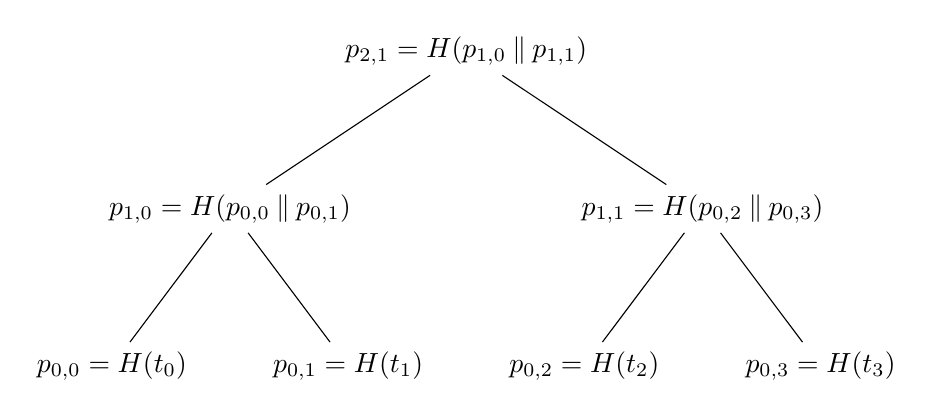
\begin{tikzpicture}[level distance=2cm,
  level 1/.style={sibling distance=6cm},
  level 2/.style={sibling distance=3cm}]
  \node {$ p_{2,1} = H(p_{1,0} \concatenate p_{1,1}) $}
    child {node {$ p_{1,0} = H(p_{0,0} \concatenate p_{0,1}) $}
      child {node {$ p_{0,0} = H(t_0) $}}
      child {node {$ p_{0,1} = H(t_1) $}}
    }
    child {node {$ p_{1,1} = H(p_{0,2} \concatenate p_{0,3}) $}
      child {node {$ p_{0,2} = H(t_2) $}}
      child {node {$ p_{0,3} = H(t_3) $}}
    };
\end{tikzpicture}

where the symbol $a \concatenate b$ means concatenating the strings $a$ and $b$. 



\subsection{Algebraic Merkle Tree}\label{algebraicMerkleTree}
An Algebraic Merkle Tree is a method for storing the sum of the value represented in the Merkle Tree. To do this, the value at each node together with the hash of the child elements is maintained as a string of JSON data. Note that in the below equations and diagrams, the quotation marks expected in the JSON format have been removed for space and clarity.

\[ Parent = \{h: H(child1 \concatenate child2),
v: child1.v+child2.v\} \]

where $h$ is the variable associated with the hash and $v$ is the variable 
associated with the stored value.

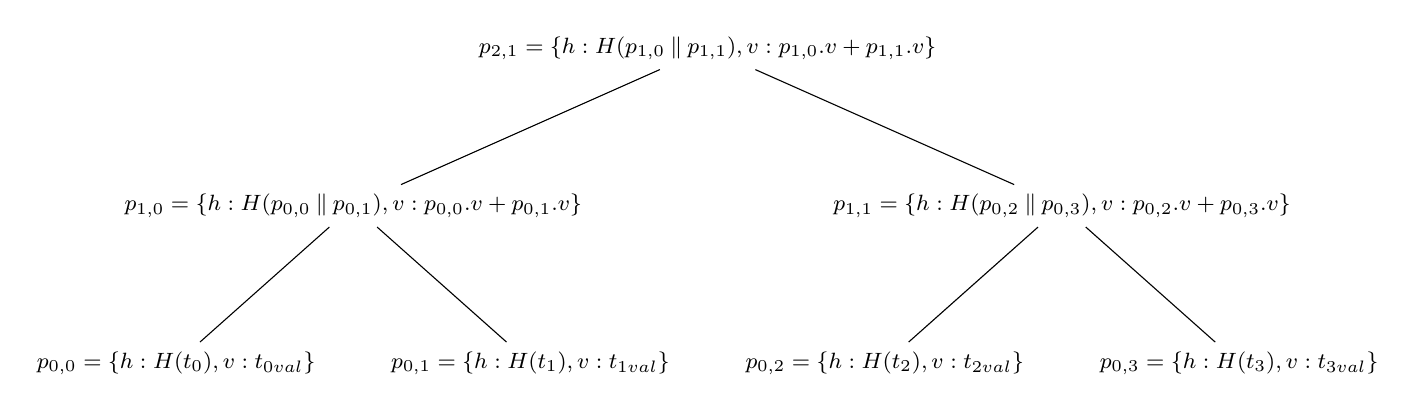
\begin{tikzpicture}[level distance=2cm,
  level 1/.style={sibling distance=9cm},
  level 2/.style={sibling distance=4.5cm}]
  \node {\footnotesize$ p_{2,1} = \{h:H(p_{1,0} \concatenate p_{1,1}),v:p_{1,0}.v+p_{1,1}.v\} $}
    child {node {\footnotesize$ p_{1,0} = \{h:H(p_{0,0} \concatenate p_{0,1}),v:p_{0,0}.v+p_{0,1}.v\}$}
      child {node {\footnotesize$ p_{0,0} = \{h:H(t_0),v:t_{0val}\}$}}
      child {node {\footnotesize$ p_{0,1} = \{h:H(t_1),v:t_{1val}\}$}}
    }
    child {node {\footnotesize$ p_{1,1} = \{h:H(p_{0,2} \concatenate p_{0,3}),v:p_{0,2}.v+p_{0,3}.v\}$}
      child {node {\footnotesize$ p_{0,2} = \{h:H(t_2),v:t_{2val}\}$}}
      child {node {\footnotesize$ p_{0,3} = \{h:H(t_3),v:t_{3val}\}$}}
    };
\end{tikzpicture}

$p_2.v$ provides the sum of all the transactions. 

Note that care must be taken when validating Algebraic Merkle Trees that all child values have a value $\geq 0$, else individuals will be able to give away more XCredits in the Merkle tree than are input to a Algebraic Merkle Tree transaction.

\subsubsection{Forming a proof}
Forming a proof for Algebraic Merkle Tree is similar to the Merkle Tree proof. At each node where the proof would ordinarily include a hash of large, ignored branch, we also include the sum of that branch, to allow the calculation of $p$ at each level. 

\subsubsection{Use cases}
The primary use case is where a single address is intending to transfer XCredits to many hidden addresses through a Merkle Tree. 

The purpose of this structure is to allow a payment aggregating organization such as a bank to efficiently make many small payments to many receivers with a single transaction.

An Algebraic Merkle Tree is trivially extended to the tracking of multiple values. 


\subsection{Sorted Merkle Tree}
A sorted Merkle Tree allows the proof not only of existence but also non-existence of data in the tree. 

Imagine you want to make it very easy to prove that an unspent transaction output has not yet been spent. to do this, you would do the following:
\begin{enumerate}
  \item Take all transactions. Sort by input address.
  \item  Use the following to calculate the parents:
\[Parent = H(\{hash: H(child1 || child2), min: child1.min, max: child2.max)\})\]
\end{enumerate}


This unspent transaction Merkle Tree could be required in a part of the block header to make it easy to prove that UTXOs have not be spent (although it is not proposed that this be include in the XCredits algorithm).

\subsubsection{Advantages over Sparse Merkle Trees}
Sparse Merkle trees are another method to prove the non-existence of elements in a Merkle Tree. By including zero elements in the Merkle Tree, the Merkle Tree can be efficiently calculated.

However, the depth of such Merkle Trees is the number of bits in the digest of the hash function being used, typically 256 bits. The impact is that for a sparse Merkle tree, each leaf that is included must be hashed roughly 255 times, which could become onerous. Similarly, when forming a proof based on a sparse Merkle tree, the size of the proof is at least $255 * 256$ bits or 65kb.

The time to calculate and recalculate proof depends on the methods used and there has been substantial investigation into this area \cite{sparseMerkleTrees1}, \cite{sparseMerkleTrees2} and \cite{sparseMerkleTrees3}.


By contrast, the number of levels necessary per entry in a Sorted Merkle Tree is
\[log_2(n)\] 
where $n$ is the number of entries in the Merkle Tree.

For Sorted Merkle Tree proof of existence in the tree, there are two extremes. Consider hashes that are numbered from zero. A hash value is between the values in position 0 and 1 will require $log_2(n)+1$ hash values to be communicated, where $n$ is the number of entries in the Merkle Tree.

% % TODO: fix maybe just remove
% \begin{tikzpicture}[level distance=2cm,
%   level 1/.style={sibling distance=4cm},
%   level 2/.style={sibling distance=2cm}]
%   \node {\footnotesize THIS REQUIRES MORE LEVELS $ p_{2,1} = H(p_{1,0} \concatenate p_{1,1}) $}
%     child {node {\footnotesize$ p_{1,0} = H(p_{0,0} \concatenate p_{0,1}) $}
%       child {node {\footnotesize$ p_{0,0} = H(t_0) $}}
%       child {node {\footnotesize$ p_{0,1} = H(t_1) $}}
%     }
%     child {node {\footnotesize$ p_{1,1} = H(p_{0,2} \concatenate p_{0,3}) $}
%       child {node {\footnotesize$ p_{0,2} = H(t_2) $}}
%       child {node {\footnotesize$ p_{0,3} = H(t_3) $}}
%     };
% \end{tikzpicture}


The worst-case scenario is if the hash value is between the maximum value of the left of the two major trees, and the minimum value of the right of the two major trees. To establish non-existence, two separate proofs must be constructed for the full height of the tree. An additional limitation is if the number of transactions is a power of two plus one, meaning a new layer must be constructed for a single transaction. As such, the worst-case scenario is approximately $2(log_2(n)+2)$, where $n$ is the number of entries in the Merkle Tree. A such, even in a worse case scenario, proof size is substantially smaller than for a Sparse Merkle Tree. 

The above approximate assumes that the difference between min and max values for the ranges in the trees are relatively small compared to the full hash, as the min and max value can truncate digits after the first few significant figures. This my not always be the case, as an attacker may deliberately choose to include hash results that are very close to one anther, forcing an increase in the number of significant figures needed to describe the ranges and hence increase the range string length in the proof. 



Sparse Merkle Trees have a significant advantage over Sorted Merkle Trees; updating a Sparse Merkle Tree requires less re-calculation as only the branches and nodes that are affected are re-calculated. In contrast, the Sorted Merkle Tree requires the entire tree to be recalculated to the right of any new entries. 





% \subsection{Full-history Merkle Tree}\label{fullhistorymerkletree}  In this section we describe a method for storing entire blockchains in Merkle  Trees by growing the Merkle Tree as new entries are added. In this regard,   Full-History Merkle Proofs are quite similar to Log Proofs. However, the main  difference is that Full-History Merkle Trees are designed to be more efficient  with its proof size and easier to determine where to find a transaction by its  transaction number.

% \begin{tikzpicture}[level distance=2cm,
%   level 1/.style={sibling distance=6cm},
%   level 2/.style={sibling distance=3cm}]
%   \node {$ p_{2,1} = H(p_{1,0} \concatenate p_{1,1}) $}
%     child {node {$ p_{1,0} = H(p_{0,0} \concatenate p_{0,1}) $}
%       child {node {$ p_{0,0} = H(t_0) $}}
%       child {node {$ p_{0,1} = H(t_1) $}}
%     }
%     child {node {$ p_{1,1} = H(p_{0,2} \concatenate p_{0,3}) $}
%       child {node {$ p_{0,2} = H(t_2) $}}
%       child {node {$ p_{0,3} = H(t_3) $}}
%     };
% \end{tikzpicture}

% It is important to note that the empty branches are not the hashes of empty  transactions. Although it is relatively trivial to calculate many levels of  empty branches and store those, it is easier from a developer perspective to  treat wholely empty branches as a simple empty string, no matter how large or  small it is.



\section{Risks and limitations}
In this section we outline some (but not all) of the technical risks that could affect the platform. There are may other risks that could affect the company X Credits Pty Ltd and the development team that are not covered here.

\subsection{Complex economic interplay}
The methods outlined in this paper are relatively simple separately. However, the convergence of these methods form a complex game with multiple players, multiple methods of earning rewards and multiple incentives. This creates a complicated interplay, with unpredictable economic and game theory outcomes. 

This is a risk to all decentralized blockchain solutions. For example, in Bitcoin it wasn't obvious from the outset that people would accept it as a means of payment, or who would mine Bitcoin on what hardware. The development of ASICs and the use of server farms filled with graphics cards brought about a level of centralization that was hard to predict ahead of time. Both of these are largely economic outcomes. Sufficient economic incentive and personal belief in the quality, stability and usefulness Bitcoin have huge impacts on the level of service quality of Bitcoin (including effective short-term denial of service at the end of 2017 as Bitcoin become greatly popular).

We expect XCredits to face many of the same economic issues that will affect the way that miners, transaction makers, transaction receivers and malicious actors behave on the system. 

\subsection{Risk of failure due to non-continuous processes}
There is risk associated with major steps in the ordinary operation of the system. For example, the shard split events represent a large change in the structure and incentives in the network. Unlike most parts of XCredits, the shard split is a non-smooth process: in step $x$, the network has 4 shards, in step $x+1$ it has 8. We have taken precautions] to help smooth this process, but the risk in this situation should not be disregarded. It is planed that the network should start with a smaller number of shards, to hopefully encourage an early shard split event, to iron out any bugs that may occur through the transition. It is also planned that there will be simulation of the transition prior to the first split event occurring. 

\subsection{Jealous attacks}
There may be people who waste more money that what is reasonable to cheat. These people, rather than trying to get more XCredits, may deliberately try to destroy XCredits a platform. The initiator of such an attack may take many forms, including nation states that see cryptocurrency as a threat to sovereign control of currency or supporters of other projects who want their project to stay on top. We have already seen many cryptocurrencies come under 51\% attack, and the recent Bitcoin Cash Wars show just how much influence a handful of individuals can have in the way that hash power is directed. The risk of this to XCredits (and any cryptocurrency) cannot be ignored. 

\subsection{Network fragmentation}
There is a risk of lock up or fragmentation due to inconsistent forking between central chain and side shards. We have provided systems that allow for side shard fork merges to occur, which should limit the possibility of this happening. However, the selection of the final central chain has many competing interests. 

A central chain miner may try to attack a side shard by including a non-broadcasted state into the central chain. This is a problem because the central chain can be considered the final say on side shards. There are a number of remedies that XCredits has available:

\begin{itemize}
  \item For the network to accept the side shard state can hence the central chain result, the miners communicating the maliciously created result will be challenged as to the side shard contents, thereby updating side shards who have been kept out of the loop about current state. It would likely take substantially more time for miners who are following that shard to communicate that they accept the shard, limiting the ability of the shard to be accepted
  \item Substantial Proof-of-Work (51\% of the central chain Proof-of-Work) is needed to force a state from the side shard to be a state of the malicious miner's choosing.   
  \item All forked blocks that can be merged successfully can be entered back into the blockchain already have their Proof-of-Work done for them, which means they can be used to create a longer chain on the shard  
  \item Even if the above fails, the transactions which cannot be merged are still available and ready to be entered back on to the blockchain. The situation would only be as bad as a transaction missing the current block in Bitcoin.
\end{itemize}


\subsection{Insufficient mining power}
In the case of collapsing price or interest in XCredits, there could be substantial reductions in the number of miners, leading to limitations in the number of nodes validating shards. XCredits does not have a method for shard merging in the event of a substantial reduction in the demand for number of transactions. Although minimum fees may mitigate this risk, there is a possibility that there could be insufficient Proof-of-Work per chain to prevent malicious activity. 







\section{Technology implementation specifics}
XCredits is intended to be a broadly distributed blockchain system, where ordinary Internet users validate the blockchain alongside large mining farms. In order to make the experience safe and easy for ordinary users, the XCredits platform is being built both as a web server and as a ``Progressive Web App".

We developed the platform as Progressive Web App, such that user can install the webpage as an App, to improve load speed and offline capability. As such, the Progressive Web App is the ultimate in ``develop once, deploy many times".

In fact, the reference implementation of the XCredits validator (XCredits Core) is built in Typescript (a typed version of JavaScript). This reference implementation is deployed to the XCredits server implementation, website implementation, Android app (using PWA architecture) and iPhone (also using PWA). 


\subsection{Platform structure}

\begin{figure}[!htb]
  \centering
  \includegraphics[page=1,width=.95\textwidth]{platform-structure} 
  \caption{XCredits Core is a generalized typescript library which is used in the ExpressJS and Angular libraries, which are used for the server and front-end interface respectively.}
  \label{fig:platform-structure}
\end{figure}
\FloatBarrier



\subsection{Globally accessible through using web standards}
Making the XCredits truly accessible by all people worldwide is a core goal of the XCredits team. To do this, the XCredits platform shouldn't be only available on high-end devices. By using the web platform as the core technology, XCredits can be sent, received and validated on low-cost devices. 


\subsection{Security through the web sandbox}
The advantage of using a PWA is not just its ease of development. As PWAs operate in a web sandbox, PWAs are safer for the user. Many cryptocurrencies have miners which you need to download, install into your computer, then give full hard drive read and write access. As the user has already self-identified to the software developer that they are interested in crypto, they have put themselves at enormous risk of being hacked and losing private keys stored on their hard drive. Even if the user does not store their private keys on that computer, cryptocurrency mining software is much more likely to be malware as a result, which could reduce participation in citizen mining.

As XCredits miners can be run safely in a web sandbox, users will be more likely to begin mining on XCredits with home machines. This will substantially improve the security and finality of XCredits as a blockchain.


\subsection{Open source}
The full source of XCredits Platform is released under an MIT License and with no patents claimed by XCredits (although XCredits makes no guarantee that the source does not violate another party's patents or other intellectual property). Please feel free to use, adapt, and extend XCredits. 


\glsaddall

\printglossaries


\begin{thebibliography}{9}
  \bibitem{SatoshiPaper} 
    Satoshi Nakamoto
    \textit{Bitcoin: A Peer-to-Peer Electronic Cash System},
    \\\texttt{http://bitcoin.org/bitcoin.pdf}, 2008.

  \bibitem{reusablePoW}
    Hal Finney
    \textit{Reusable Proofs of Work}
    \\\texttt{https://web.archive.org/web/20071222072154/http://rpow.net/}, 2007.
  
  \bibitem{ethereumshardingFaqs}
    Ethereum Foundation
    \textit{Ethereum Sharding FAQs}
    \\\texttt{https://github.com/ethereum/wiki/wiki/Sharding-FAQs}, 2018.

  \bibitem{ethereumResearchCompendium}
    Ethereum Foundation
    \textit{Ethereum Sharding Research Compendium}
    \\\texttt{https://notes.ethereum.org/oa8wCimaTPGBl2nHuBTXWQ}, 2018

  \bibitem{onSlowAndFastBlockTimes}
    Vitalik Buterin
    \textit{On Slow and Fast Block Times}
    \\\texttt{https://blog.ethereum.org/2015/09/14/on-slow-and-fast-block-times/}, 2015

  \bibitem{towardA12SecondBlockTime}
    Vitalik Buterin
    \textit{Toward a 12-second Block Time}
    \\\texttt{https://blog.ethereum.org/2014/07/11/toward-a-12-second-block-time/}, 2014

  \bibitem{sparseMerkleTrees1}
    Rasmus Dahlberg, Tobias Pulls, and Roel Peeters
    \textit{Efficient Sparse Merkle Trees Caching Strategies and Secure (Non-)Membership Proofs
    }
    \\\texttt{https://eprint.iacr.org/2016/683.pdf}

  \bibitem{sparseMerkleTrees2}
    Markus Knecht, Willi Meier, and Carlo U. Nicola
    \textit{A space– and time–efficient Implementation of the Merkle Tree
    Traversal Algorithm}
    \\\texttt{https://arxiv.org/pdf/1409.4081.pdf}, 2014

  \bibitem{sparseMerkleTrees3}
    Faraz Haider
    \textit{Compact Sparse Merkle Trees}
    \\\texttt{https://eprint.iacr.org/2018/955.pdf}, 2018

  \bibitem{xspoct}
    James Jansson
    \textit{XCredits-Style Private, Off-Chain Transactions (XSPOCT)}
    \\\texttt{https://github.com/XCredits/xcredits-whitepapers/blob/master/xspoct.md}, 2018
  % Controlled supply - Bitcoin Wiki
  % https://en.bitcoin.it/wiki/Controlled_supply

\end{thebibliography}


\end{document}